\documentclass[
11pt,%
tightenlines,%
twoside,%
onecolumn,%
nofloats,%
nobibnotes,%
nofootinbib,%
superscriptaddress,%
noshowpacs,%
centertags]%
{revtex4}
\usepackage{ljm}
\usepackage{listings}
\usepackage{amsmath}

\lstset{
language=C++,
basewidth=0.5em,
xleftmargin=45pt,
xrightmargin=45pt,
basicstyle=\small\ttfamily,
keywordstyle=\bfseries\underbar,
numbers=left,
numberstyle=\tiny,
stepnumber=1,
numbersep=10pt,
showspaces=false,
showstringspaces=false,
showtabs=false,
frame=trBL,
tabsize=2,
captionpos=t,
breaklines=true,
breakatwhitespace=false,
escapeinside={\%*}{*)}
}

\begin{document}

\titlerunning{solving nonlinear equations}
\authorrunning{Bagrov, Rybakov}

\title{Selection of a method for solving nonlinear equations in shallow-water icing model implementation}

\author{\firstname{A.~D.}~\surname{Bagrov}}
\email[E-mail: ]{andrey.bagrov@yandex.ru}
\affiliation{Joint Supercomputer Center of the Russian Academy of Sciences -- branch of Scientific Research Institute of System Analysis of the Russian Academy of Sciences, Leninsky prospect 32a, Moscow, 119334, Russia}

\author{\firstname{A.~A.}~\surname{Rybakov}}
\email[E-mail: ]{rybakov.aax@gmail.com}
\affiliation{Joint Supercomputer Center of the Russian Academy of Sciences -- branch of Scientific Research Institute of System Analysis of the Russian Academy of Sciences, Leninsky prospect 32a, Moscow, 119334, Russia}

\firstcollaboration{(Submitted by TODO)} % Add if you know submitter.
%\lastcollaboration{ }

\received{TODO}

\begin{abstract}
Ice accretion simulation on aircraft profiles during their flight in an air stream containing supercooled water droplets is an extremely important task for flight safety, since the form of accreted ice significantly affects flight characteristics.
In one of the models for solving the problem, the shallow-water icing model (SWIM), the problem of solving nonlinear equations with one variable plays a central role in numerical simulation.
Since this problem occupies the overwhelming majority of calculations time, the question of choosing the optimal method for solving nonlinear equations and optimizing these methods becomes especially acute.
This article describes the analysis of the use of various methods for solving nonlinear equations in the implementation of the SWIM solver, taking into account the features of the equations being solved, which led to a significant acceleration of the computational codes when performing calculations on JSCC RAS supercomputers.
\end{abstract}

\subclass{65H05, 65Y20} % Enter 2010 Mathematics Subject Classification.

\keywords{nonlinear equations, shallow-water icing model, bisection method, Newton's method, Brent's method}

\maketitle

\section{Introduction}

At present, there are a lot of computational codes used for numerical simulation of icing on a streamlined body surface.
Some of the most popular packages for this task are Lewice \cite{Wright} and ONERA.
In this article, we will not discuss the features of these calculation packages and the differences between them, but consider only the implementation of the SWIM solver, described in detail in \cite{Bourgault}.
When performing computer simulation of the icing process of a surface in a free stream, the shallow-water icing model performs a simultaneous calculation of the ice accretion and the flow of a liquid film over the surface of the streamlined body. This takes into account the loss of moisture on the surface of the body, evaporation of water or sublimation of ice from the surface of the body, the flow of a liquid film over the surface with its partial freezing, as well as the overflow of heat fluxes between the body and the surface and between the surface and the surrounding air.

Numerical calculations are performed on a surface computational mesh, consisting of individual cells, while in each cell of the surface, the mass conservation law must be fulfilled, written in the following form:

\begin{equation}
\rho_w \left[ \frac{\partial h_f}{\partial t} + \operatorname{div}(\overline{u} h_f) \right] = U_{\infty} LWC \beta - \dot m_{evap} - \dot m_{ice}
\end{equation}

In this formula, $\rho_w$ is the density of water, $h_f$ is the height of the water film on the surface, $\overline{u}$ is the velocity of the water film, $U_{\infty}$ is the speed of the free stream, $LWC$ is the liquid water content in the free stream, $\dot m_{evap}$ is the specific rate of evaporation or sublimation from the surface of the streamlined body, $\dot m_{ice}$ is the specific rate of ice mass increasing.

In addition, the law of conservation of energy is fulfilled in each cell:

\begin{equation}
\begin{aligned}
& \rho_w \left[ \frac{\partial h_f C_w \tilde{T}}{\partial t} + \operatorname{div}(\overline{u} h_f C_w \tilde{T}) \right] = \left[ C_w \tilde{T}_{d,\infty} + \frac{||\overline{u}_d||^2}{2} \right] \times U_{\infty} LWC \beta
\\
& - \frac{1}{2}(L_{evap} + L_{subl}) \dot m_{evap} + (L_{fusion} - C_{ice} \tilde{T}) \dot m_{ice} + \sigma (T_{\infty}^4 - T^4) + \dot Q_h + \dot Q_{cond}
\end{aligned}
\end{equation}

In this formula, $C_w$ is the specific heat of water, $\tilde{T}$ is the cell temperature in degrees Celsius, $\tilde{T}_{d,\infty}$ is the temperature of the inpingement droplets in degrees Celsius, $\overline{u}_d$ is the speed of droplets falling onto the surface, $L_{evap}$ is the latent heat of water evaporation, $L_{subl}$ is the latent heat of ice sublimation, $L_{fusion}$ is the latent the heat of ice melting, $C_{ice}$ is the heat capacity of ice, $\sigma$ is the Boltzmann constant, $T_{\infty}$ is the free stream temperature in kelvin, $T$ is the cell temperature in kelvin, $\dot Q_h$ is the specific value of the heat flux received from the air, $\dot Q_{cond}$ is the specific value of the heat flux entering the cell from the surface.

For the numerical solution of the given system of equations, it is necessary to discretize it in time and space, as shown in \cite{Beaugendre}.
After that, we obtain a system of two difference equations, which include three unknown variables: surface temperature $\tilde{T}$, height of water film $h_f$ and height of ice $h_{ice}$.

Also, when solving the system of equations, the compatibility conditions must be satisfied, written in the form

\begin{equation}
\begin{cases}
h_f \ge 0\\
\dot m_{ice} \ge 0\\
h_f \tilde{T} \ge 0\\
\dot m_{ice} \tilde{T} \le 0
\end{cases}
\end{equation}

\begin{figure}[h]
\setcaptionmargin{5mm}
\onelinecaptionstrue
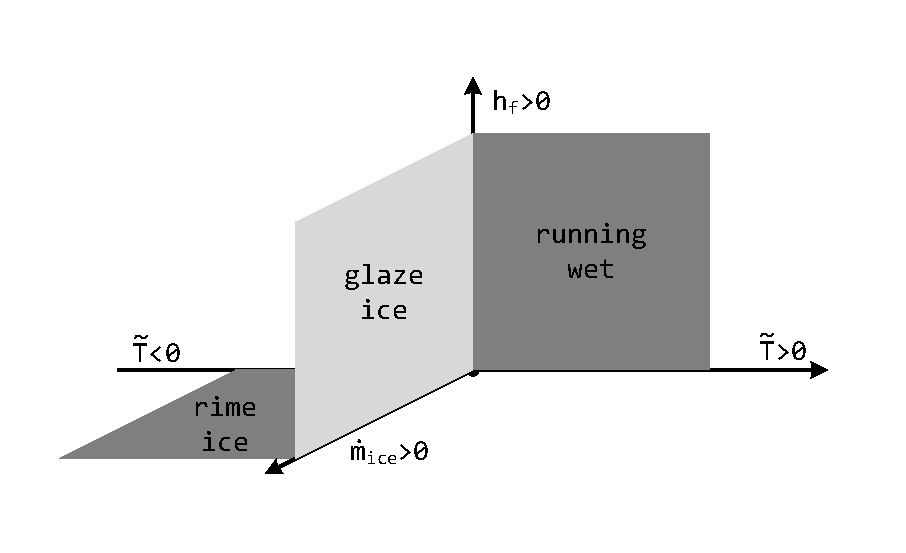
\includegraphics[width=0.7\textwidth]{pics/surface.pdf}
\captionstyle{normal}\caption{The space of solutions of the system of equations for the mass and heat balance of the cell.}\label{fig:surface}
\end{figure}

Despite the fact that there are more unknowns in the equation than the equations themselves, the system is still solved, since these variables are not completely independent.
The solution is taken from the condition that the cell can be in one of three states.
The first state is running wet, it is reached when there is no ice in the cell and a liquid film flows.
In this case, the temperature cannot be negative.
The second state is glaze icing, if both ice and water are present in the cell at the same time.
In this case, the temperature is zero degrees Celsius.
And finally, in the third case, at a negative temperature, the cell cannot contain water and only ice is present.
The general solution space is shown in Fig.~\ref{fig:surface}.

\section{Features of the equations being solved}

Для состояния ячейки glaze ice система уравнений, состоящая из уравнения массового баланса и уравнения теплового баланса, вырождается в простую систему линейных уравнений с двумя неизвестными (высота водяной пленки и высота ледяного нароста).
Решение такой системы уравнений не представляет сложностей.
Для двух оставшихся состояний ячейки (running wet, rime ice) описанная система уравнений сводится к одному нелинейному уравнению с одной переменной (неизвестной в данном случае является температура ячейки).
При этом в нелинейное уравнение входят такие физические величины как удельная теплоемкость воды, льда и воздуха ($C_w$, $C_{ice}$, $C_a$), скрытое тепло испарения и сублимации ($L_{ev}$, $L_su$), а также динамическая вязкость воды ($\mu_w$).
Данные величины не являются константами, а сами зависят от температуры нелинейным образом.
На Fig.~\ref{fig:ph_graphics_h} показана кусочно-линейная интерполяция данных физических величин, выполненная по их табличным значениям.

\begin{figure}[h]
\setcaptionmargin{5mm}
\onelinecaptionstrue
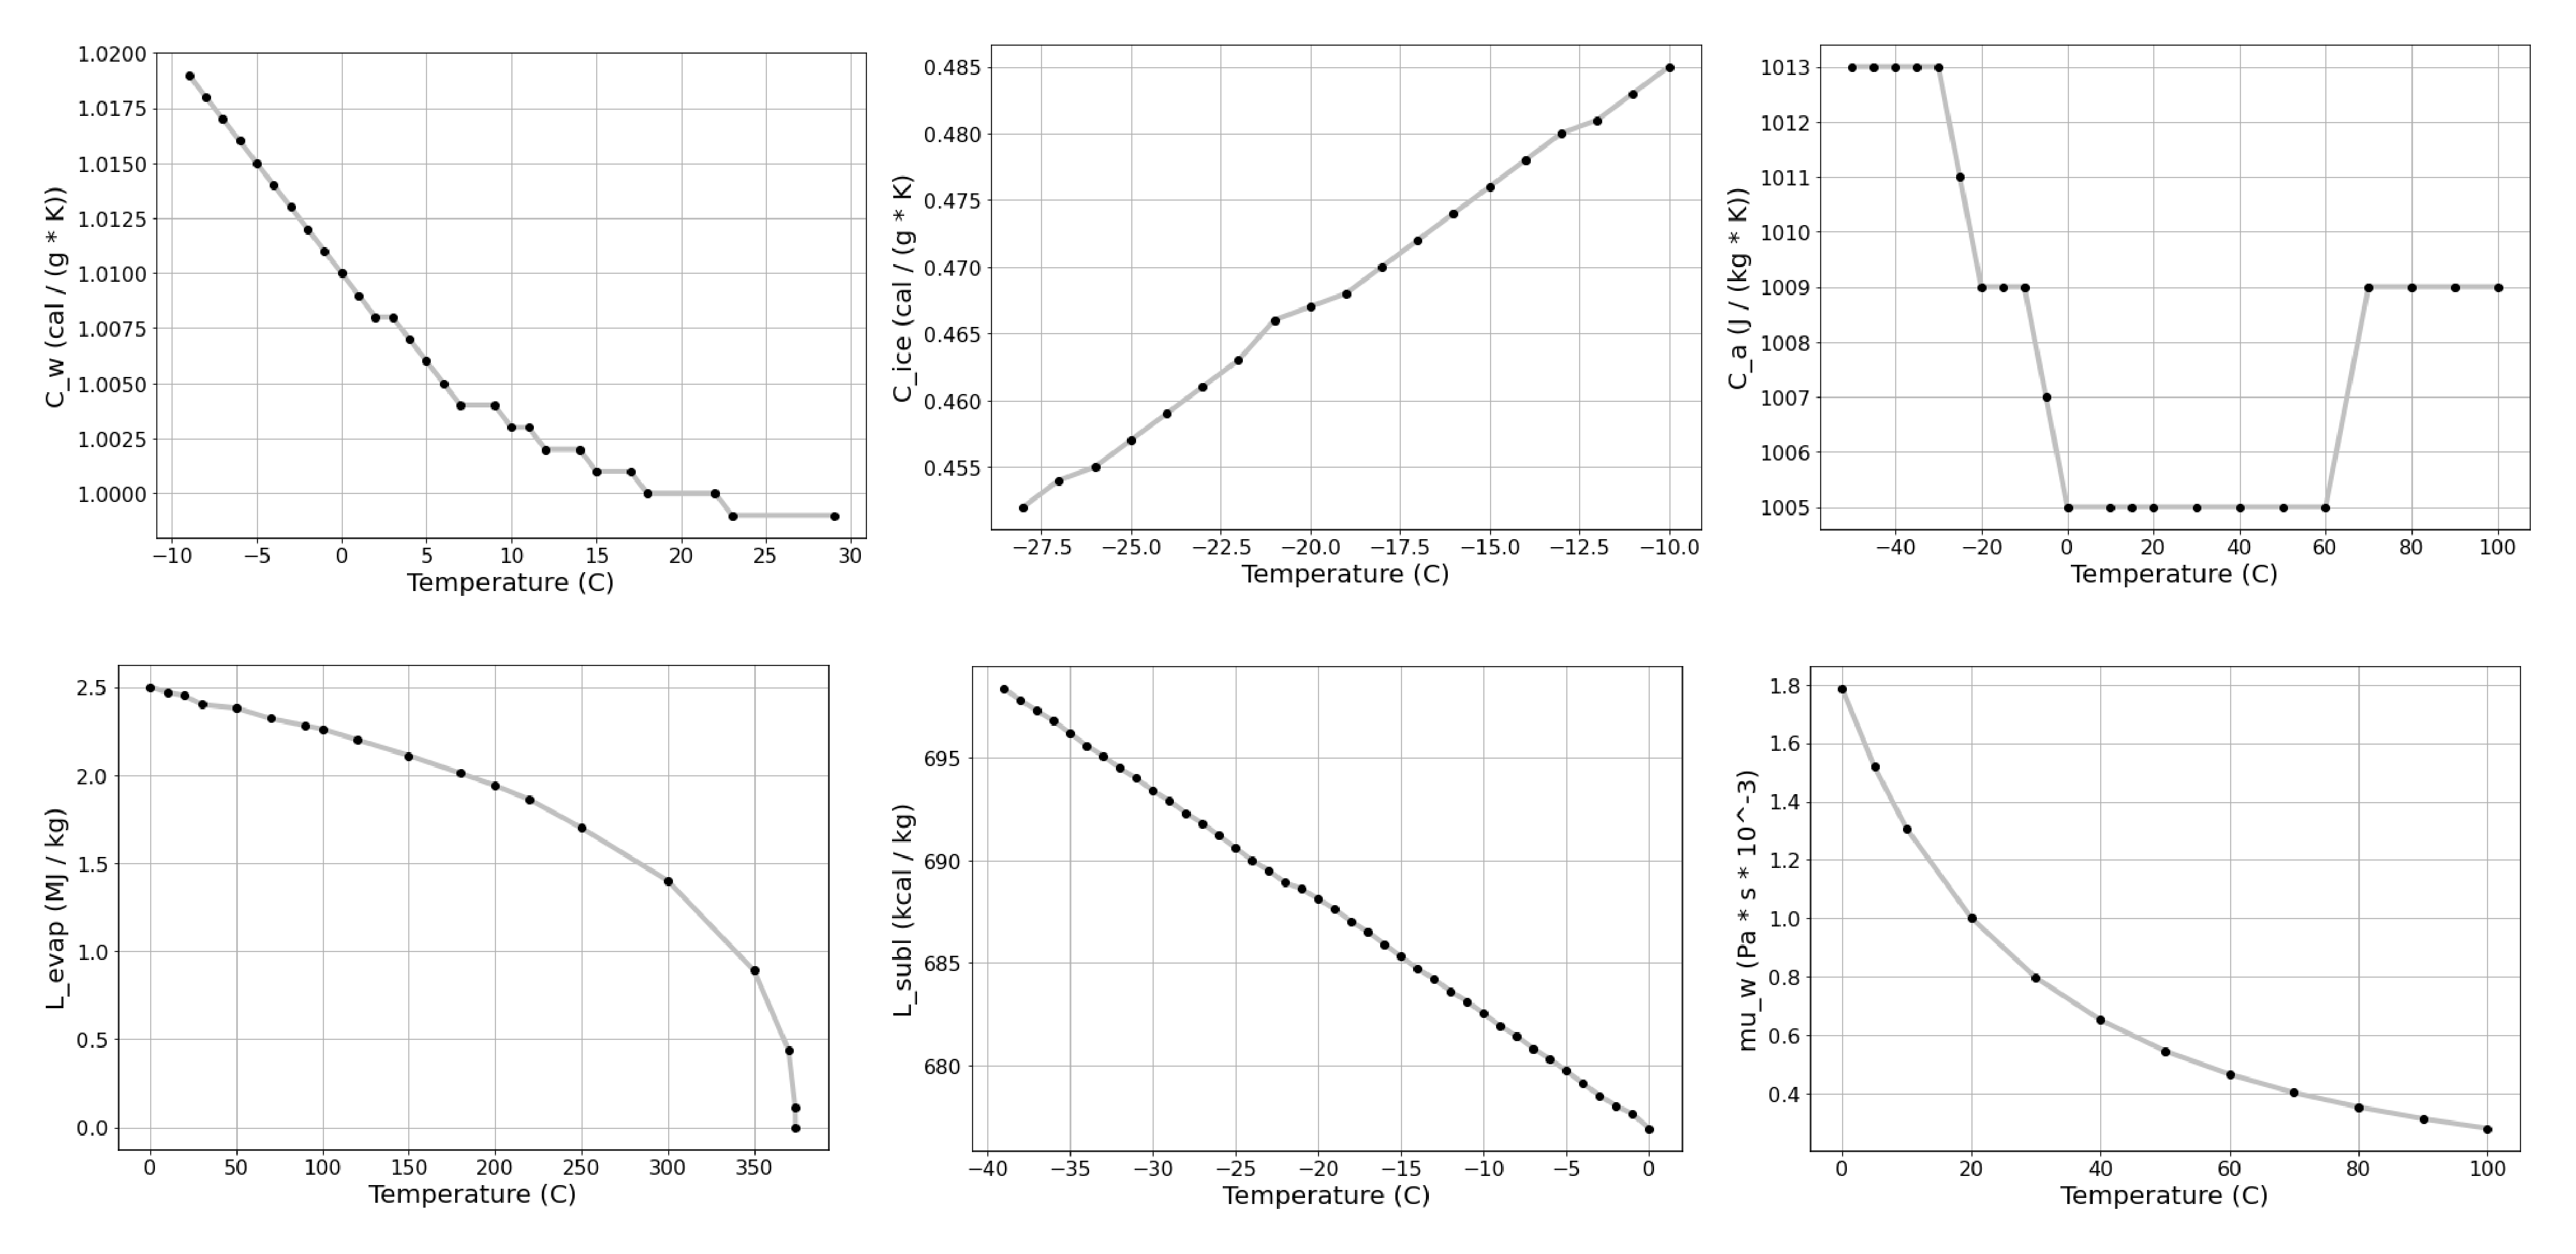
\includegraphics[width=1.0\textwidth]{pics/ph_graphics_h.pdf}
\captionstyle{normal}\caption{Зависимости физических величин от температуры.}\label{fig:ph_graphics_h}
\end{figure}

В процессе выполнения расчетов в масштабах всей поверхности были использованы неструктурированные расчетные сетки с характерным числом ячеек $10^5$, характерное время счета составляет $10^3$ секунд, характерный шаг по времени $10^{-3}$ секунды.
В общем случае на каждом шаге по времени требуется решать нелинейное уравнение от 0 до 2 раз (будем считать, что в среднем 1 раз).
Итого, получаем, что характерное количество запусков решения нелинейного уравнения в процессе запуска типовой расчетной задачи составляет $10^11$ штук.
Такое количество запусков решения нелинейных уравнений является существенных даже при условии распараллеливания вычислений с помощью MPI, OpenMP и применения векторизации программного кода.
Поэтому выбор оптимального метода решения нелинейных уравнений является критически важной задачей для повышения быстродействия программного кода.

При тестировании различных методов решения нелинейных уравнений были собраны профили функций ($f(x)$), для которых требуется найти решение.
Многообразие данных профилей продемонстрировано на Fig.~\ref{fig:dq}.
На этой иллюстрации построены графики семейства функций $f(x)$ для взятых случайным образом ячеек расчетной сетки для случайных моментов времени и для разрешения различных состояний ячеек.

\begin{figure}[h]
\setcaptionmargin{5mm}
\onelinecaptionstrue
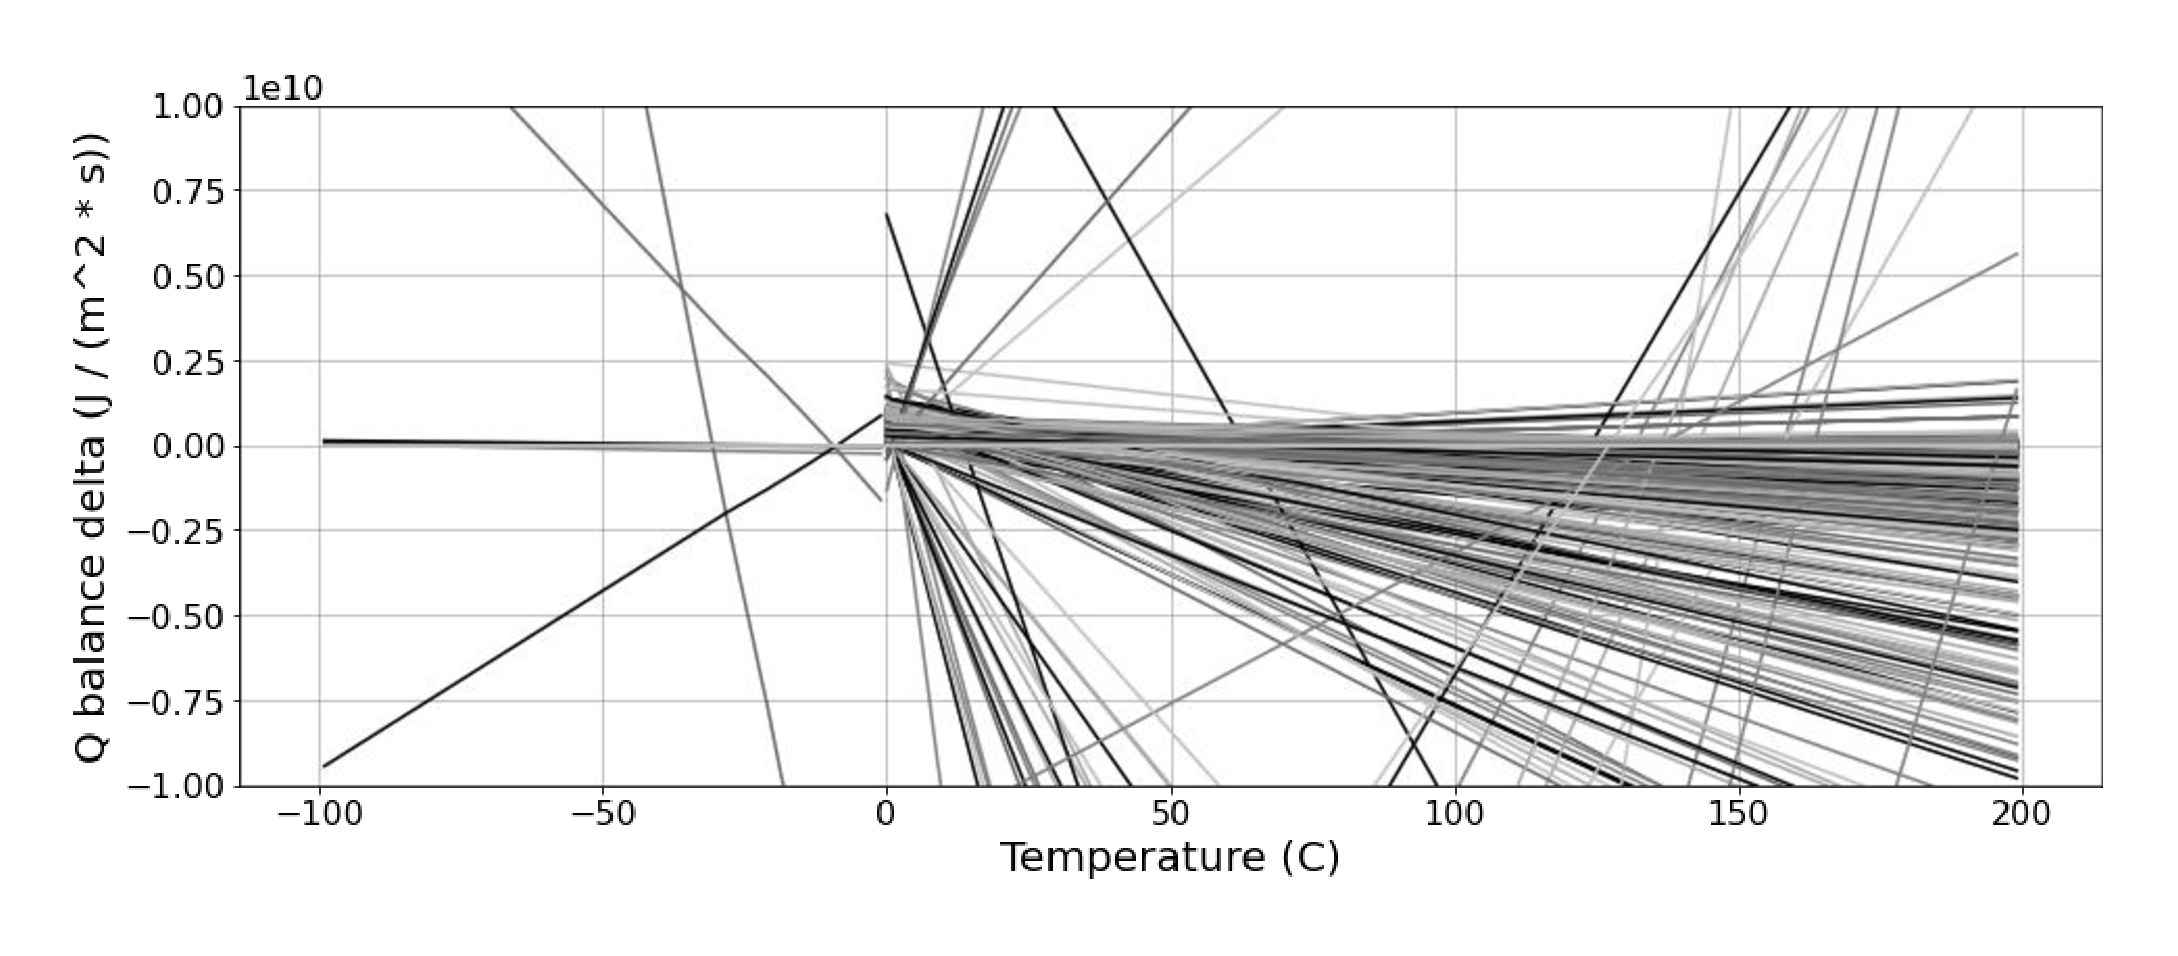
\includegraphics[width=1.0\textwidth]{pics/dq.pdf}
\captionstyle{normal}\caption{Графики функций, представляющих решаемые нелинейные уравнения.}\label{fig:dq}
\end{figure}

Из приведенной иллюстрации может создаться впечатление, что в основном уравнения решались для состояний ячейки running wet (так как область построения графиков $x > 0$ плотно заполнена графиками).
Однако это впечатление ошибочно, просто большинство графиков функций $f(x)$ для состояния ячейки rime ice при данном масштабе сильно прижаты с оси $OX$ и сливаются в один график.
На Fig.~\ref{fig:dq_rime_wet} приведены графики функций для разрешения состояний ячеек rime ice (слева) и running wet (справа) раздельно и в разным масштабах.
На данных графиках можно наблюдать общий вид графиков, представляющих уравнения для разрешения данных двух состояний ячейки.

\begin{figure}[h]
\setcaptionmargin{5mm}
\onelinecaptionstrue
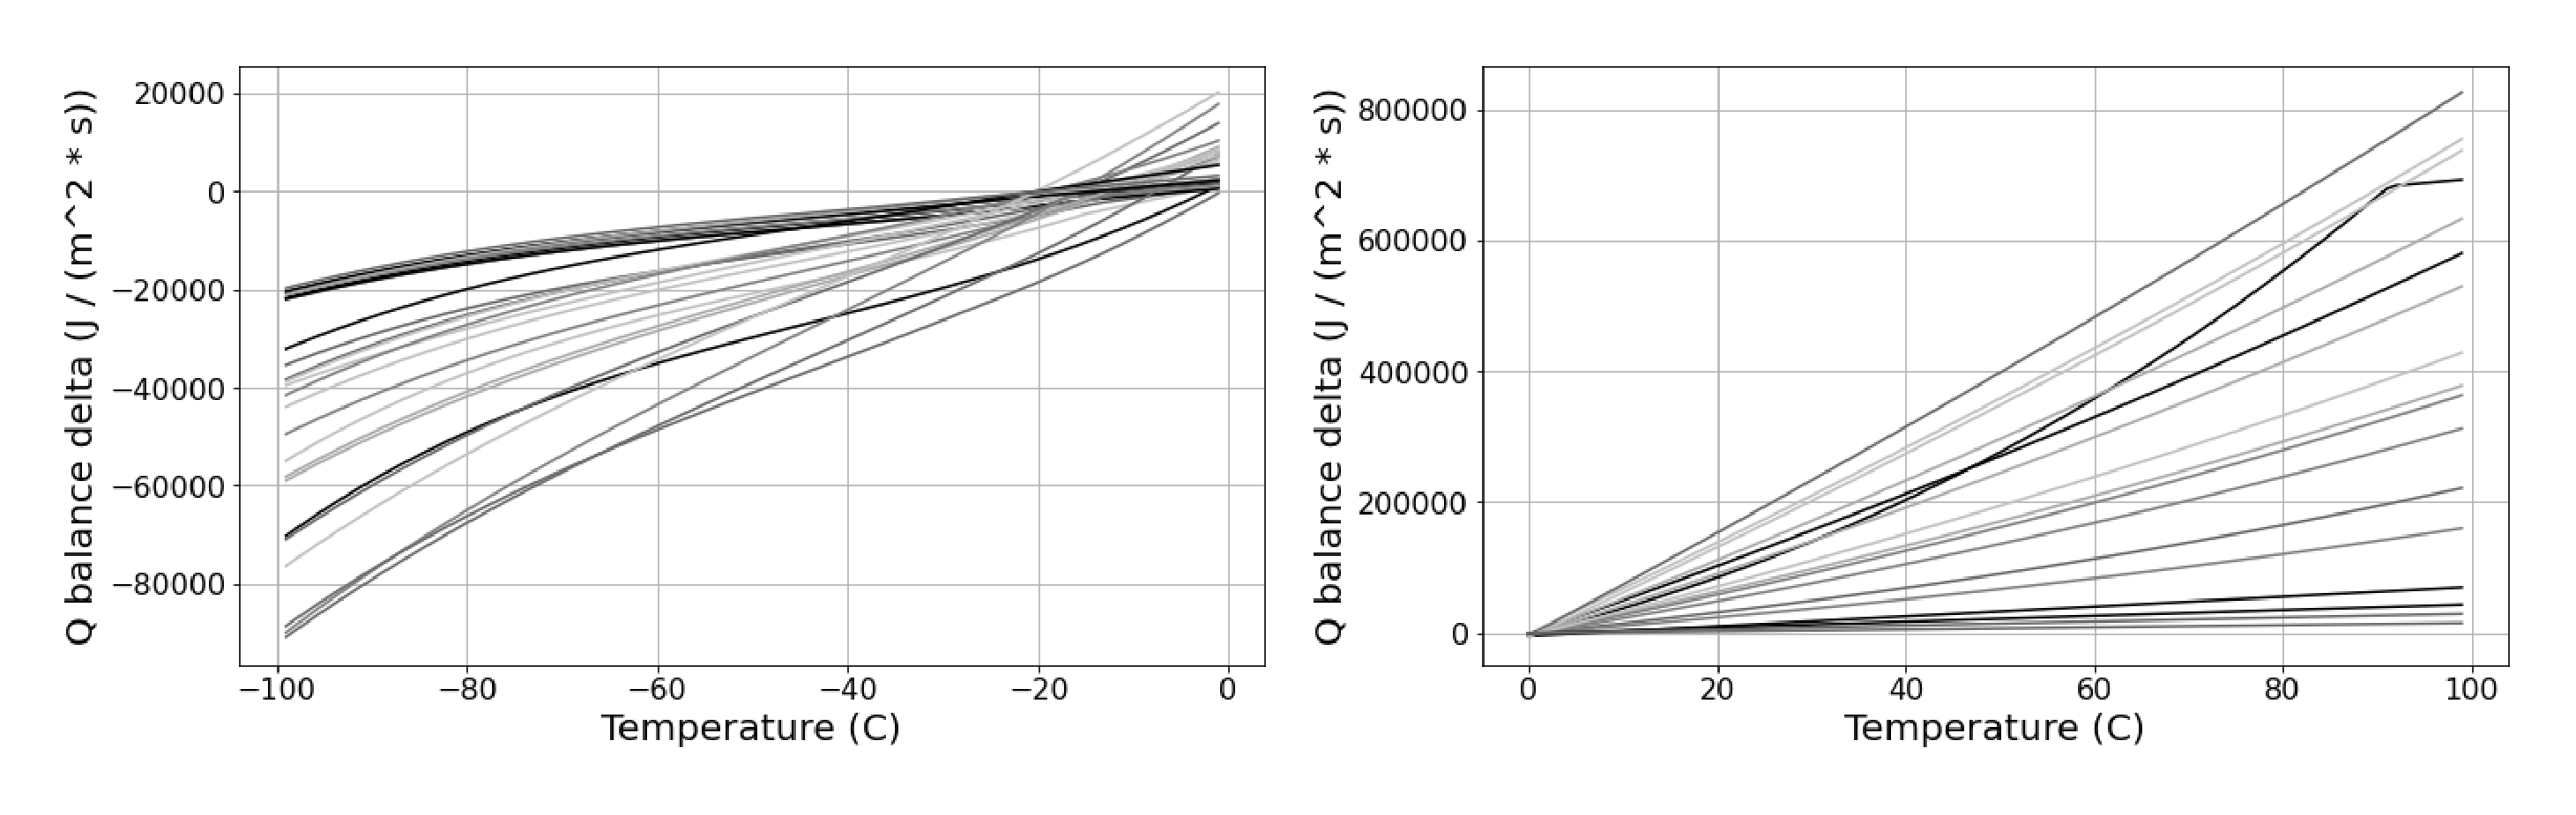
\includegraphics[width=1.0\textwidth]{pics/dq_rime_wet.pdf}
\captionstyle{normal}\caption{Семейсва графиков функций решения нелинейных уравнений при определения состояния ячеек rime ice (слева) и running wet (справа).}\label{fig:dq_rime_wet}
\end{figure}

\section{Methods of solving nonlinear equations}

Итак, мы рассматриваем решение нелинейного уравнения вида $f(x) = 0$, полученного из системы уравнений массового и теплового баланса для разрешения одного из состояний ячейки.
При выборе оптимального метода решения нелинейных уравнения для поставленной задачи использовались следующие методы: метод бисекций, метод хорд, метод Ньютона, метод Брента.
Уравнения решались в температурном интервале $x \in [-100, 200]$, для решаемых уравнений было выполнено условие $f(a) f(b) < 0$.

Метод бисекций рассматривался в качестве эталона для сравнения с другими методами, так как ясно, что он является наиболее медленным, зато гарантированно сходится при любых начальных условиях и любом виде анализируемой функции.
В процессе решения нелинейного уравнения методом бисекции интервал поиска на каждой итерации решения делится на два равные интервала, из которых выбирается один, для которого продолжает выполняться условие разнознаковости функции на концах интервала.

Метод хорд сход по смыслу с методом бисекций, однако на каждой итерации решения уравнения интервал поиска корня делится не на две равные части.
Точкой деления интервала поиска на два новых интервала определяется как пересечение оси $OX$ c отрезком $[(a, f(a)), (b, f(b))]$.
Данный метод в большинстве случаев приводит к более быстрому решению уравнения, однако возможны профили функций, для которых применение метода хорд может привести к катастрофическому замедлению процесса поиска корня.

На Fig.~\ref{fig:chords-newton} представлены схемы поиска корней нелинейного уравнения с помощью методов хорд и метода Ньютона.

\begin{figure}[h]
\setcaptionmargin{5mm}
\onelinecaptionstrue
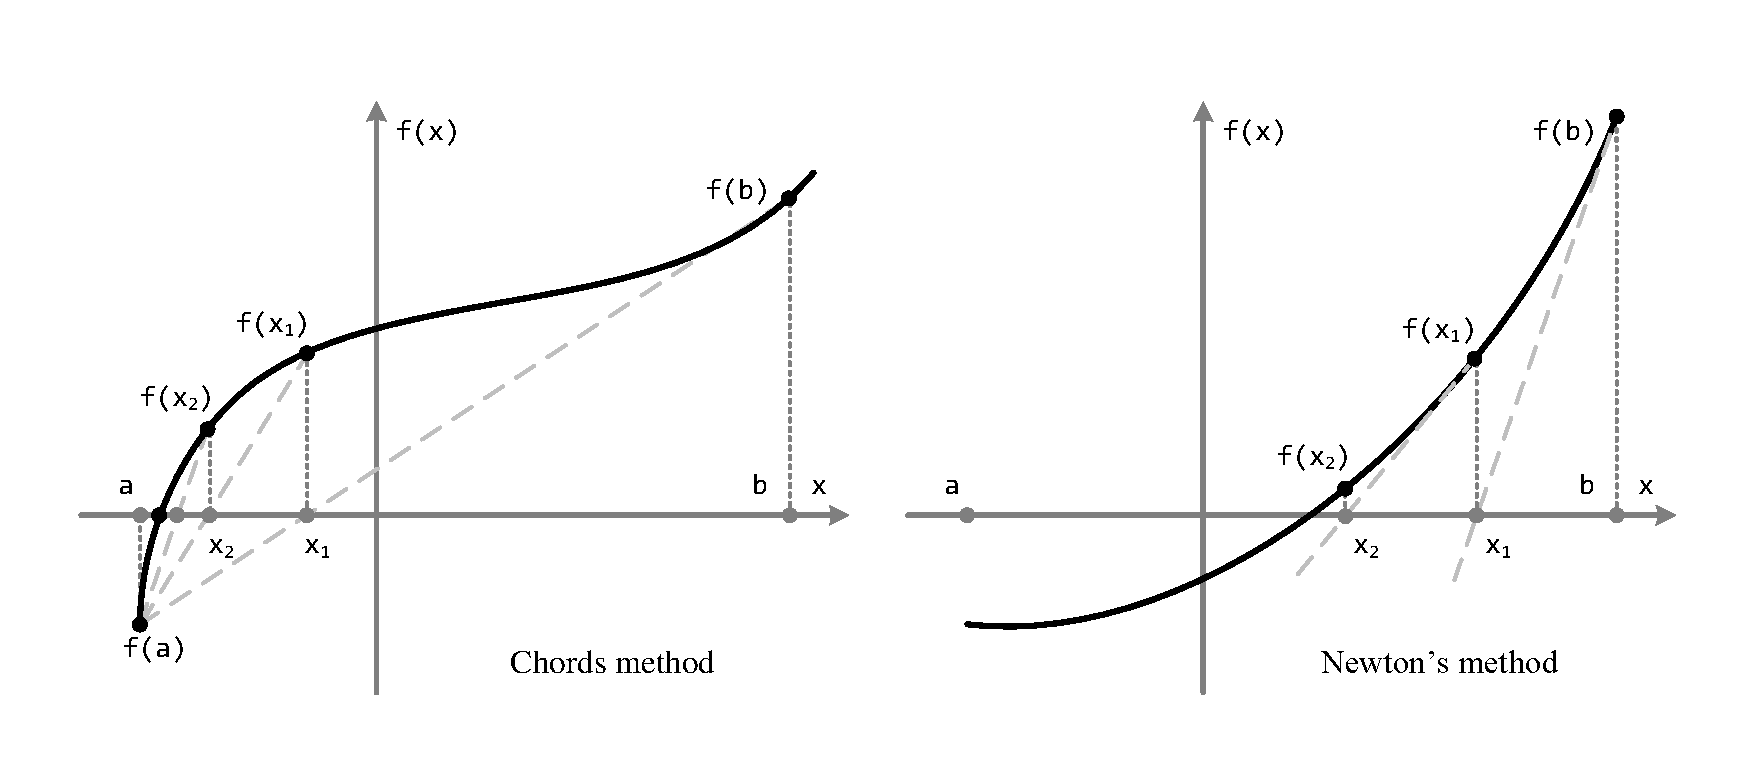
\includegraphics[width=1.0\textwidth]{pics/chords-newton.pdf}
\captionstyle{normal}\caption{Схемы поиска корня нелинейного уравнения методом хорд и методом Ньютона.}\label{fig:chords-newton}
\end{figure}

В методе Ньютона корень уравнения ищется начиная с некоторой точки (на Fig.~\ref{fig:chords-newton} начинаем с точки $b$).
Из данной точки проводится касательная до пересечения с осью $OX$ (что соответствует вычислению разностной производной с требуемым порядком точности) в некоторой точке $x_i$, которая и становится новым значением - кандидатом на корень уравнения.
Данный метод крайне эффективен для поиска корней уравнений, представленных, например, выпуклыми функциями, однако существуют профили функций, для которых метод Ньютона неприменим или может работать крайне медленно.

Метод Брента является модифицированным методом Деккера, который, в свою очередь, является объединением метода деления пополам с методом секущих.
В методе Деккера на каждой итерации происходит попытка применить метод хорд для сужения интервала поиска корня, а при невозможности применения метода хорд выполняется применение одной итерации метода бисекции.
В методе Брента осуществляется похожий синтез метода хорд и метода бисекций.
В этом методе также выполняется попытка применения метода хорд, а при снижении скорости стягивания интервала поиска корня применяются разовые итерации метода бисекций.
Кроме этого, линейная интерполяция в методе хорд заменена обратной квадратичной интерполяций.

\section{Numerical experiments}

\begin{figure}[h!]
\setcaptionmargin{5mm}
\onelinecaptionstrue
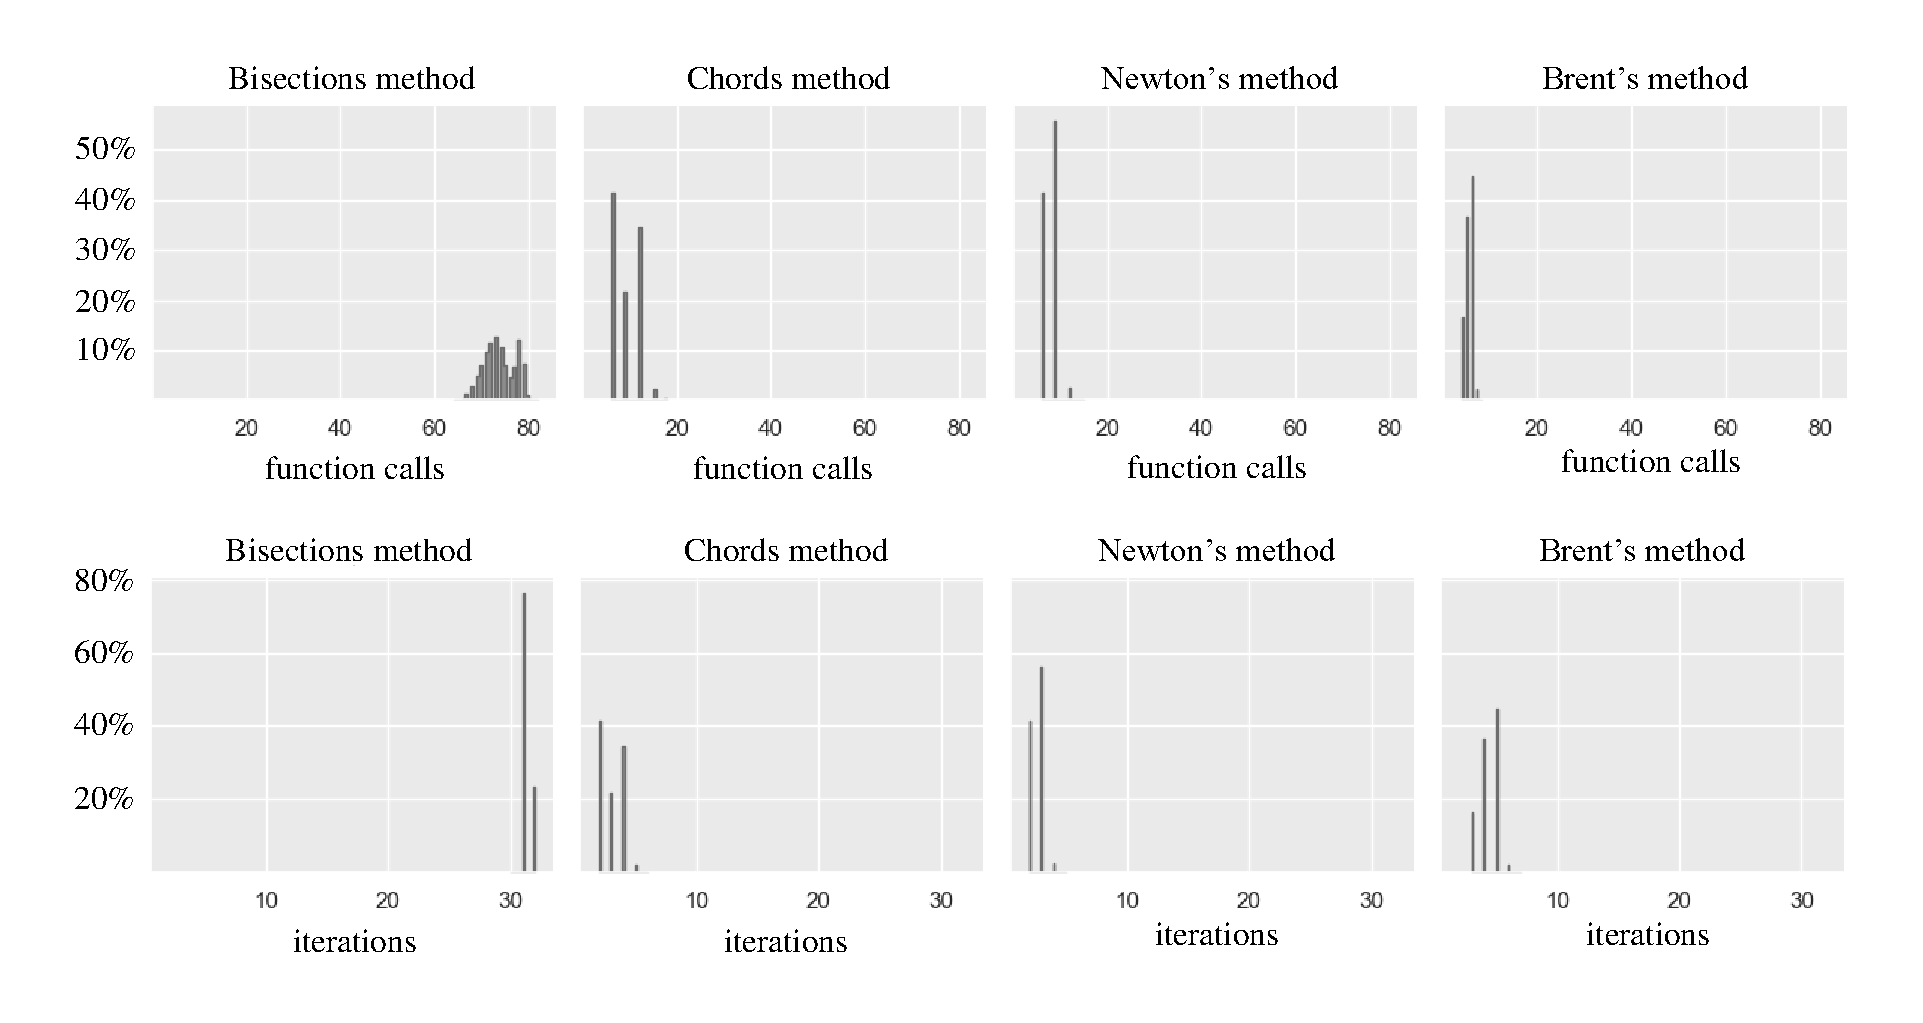
\includegraphics[width=1\textwidth]{pics/stat.pdf}
\captionstyle{normal}\caption{Статистика количеств вызово функции $f(x)$ и итераций решения нелинейного уравнения}\label{fig:stat}
\end{figure}

Для анализа использования различных методов решения нелинейных уравнений по запуску на расчетных типовых задачах, решаемых при различных температурах свободного потока была собрана статистика по количеству итераций решения уравнений и общему количеству вызовов функций $f(x)$, необходимых для решения данных уравнений.
На Fig.~\ref{fig:stat} представлена сводная статистика.
В Table~\ref{tab:stat} собраны данные по среднему количеству итераций и вызовов функций при использовании всех описанных методов решения уравнений.

\begin{table}[h!]
\label{tbl:supercomputers}
\setcaptionmargin{0mm}
\onelinecaptionsfalse
\captionstyle{flushleft}
\caption{Статистика применения различных методов решения нелинейных уравнений.}\label{tab:stat}
\bigskip
\begin{tabular}{|c|c|c|}
\hline
Method & Avg. func calls & Avg. iterations \\
\hline
bisections & 78,8 & 31,3 \\
\hline
chords & 11,2 & 3,7 \\
\hline
Newton's & 10,1 & 3,3 \\
\hline
Brent's & 5,5 & 4,5 \\
\hline
\end{tabular}
\label{tab:supercomputers}
\end{table}

Стоит отметить, что общее количество вызовов функции $f(x)$ в ходе решения уравнений является наиболее важной характеристикой с точки зрения эффективности метода решения нелинейного уравнения, так как на это тратится вычислительное время.
Исходя из данных, представленных на Fig.~\ref{fig:stat} и Table~\ref{tab:stat}, можно увидеть, что метод Ньютона требует для решения рассматриваемых нелинейных уравнений в среднем всего 3,3 итерации.
Однако с точки зрения производительности метод Брента в процессе своей работы выполняет почти в два раза меньше вызовов функции $f(x)$, что приводит к практически двукратному ускорению скорости расчетов относительно метода хорд и метода Ньютона.

\section{Conclusion}

В работе была рассмотрена постановка задачи расчета физических процессов в рамках shallow-water icing model.
Ядром работы данного решателя является решение нелинейного уравнения с одной неизвестной.
Решение данной задачи занимает подавляюще большую часть всех вычислений решателя, поэтому выбор оптимального метода решения нелинейного уравнения крайне важен.
В процессе выполнения исследований были собраны профили функций, для которых требуется решать нелинейные уравнений и на собранных данных проанализированы следующие методы: метод бисекций, метод хорд, метод Ньютона и метод Брента.
С точки зрения среднего количества итераций поиска корня уравнения наиболее выгодным оказался метод Ньютона.
Однако, общее количество вызовов функции $f(x)$ оказалось в среднем ниже при использовании метода Брента, что обуславливает оптимальность данного метода для применения в решателе shallow-water icing model.

\begin{acknowledgments}
The work has been done at the JSCC RAS as part of the state assignment for the topic 0580-2021-0016.
The supercomputer MVS-10P OP, located at the JSCC RAS, was used during the research.
\end{acknowledgments}

\begin{thebibliography}{99}

\bibitem{Wright}
\refitem{article}
W.~W.~Wright, P.~Struck, T.~Bartkus, G.~Addy, {\it ``Recent Advances in the LIWICE Icing Model''}, SAE Technical Paper (2015).

\bibitem{Bourgault}
\refitem{article}
Y.~Bourgault, H. Beaugendre, W. G. Habashi, {\it ``Development of a Shallow-Water Icing Model in FENSAP-ICE''}, Journal of Aircraft, Vol. 37, No. 4, 640--646 (2000).

\bibitem{Beaugendre}
\refitem{misc}
H.~Beaugendre, {\it ``A PDE-Based Approach to In-Flight Ice Accretion''}, A thesis of the degree of Doctor of Philosophy, Department of Mechanical Engineering, McGill University, Montreal, Qu\'ebec (2003).

\bibitem{Dekker}
\refitem{article}
Brent, R.P.. Finding a zero by means of successive linear interpolation. : London, 1969.

\bibitem{Brent}
\refitem{book}
Brent, R.P.. Algorithms for minimization without derivatives. : Prentice-Hall, 1973.

\bibitem{Press}
\refitem{book}
William H. Press, Saul A. Teukolsky, William T. Vetterling, and Brian P. Flannery. 2007. Numerical Recipes 3rd Edition: The Art of Scientific Computing (3rd. ed.). Cambridge University Press, USA.


\end{thebibliography}

\end{document}
